% Makros zur Kompatibilitaet mit Onlinemodul: 
 \providecommand{\MoIl}[1][]{\mbox{}#1]\mathopen{}} 
 \providecommand{\MoIr}[1][]{#1[\mbox{}} 
 \providecommand{\MIntvlSep}{;} 
 \providecommand{\MElSetSep}{\, ; \, } 
 \begin{MAufgabe}{Lineare Betrags(un)gleichungen}{vr, 2016, MaTeX}
L\"osen Sie die Gleichung
$$
 \MDS 4\left| x + 2 \right|2 - 4\, x= 4 \left| 4\, x + 1 \right| +4\, x - 3
$$  

\ifLsg\MLoesung

Im ersten Schritt k\"onnen die Terme au\ss{}erhalb der Betragszeichen zusammengefasst werden:

\begin{align*} 
 4\left| x + 2 \right|2 - 4\, x= 4 \left| 4\, x + 1 \right| +4\, x - 3\\ 
\Leftrightarrow4\, \left|x + 2\right| - 8\, x - 4\, \left|4\, x + 1\right| + 5= 0 
 \end{align*}

F\"ur diese Gleichung haben wir 4 F\"alle zu unterscheiden: 
\begin{enumerate}
\item $ \MDS 
\begin{cases} 
 0 \leq x + 2\\ 
0 \leq 4\, x + 1
 \end{cases}
\Leftrightarrow - \frac{1}{4} \leq x\Leftrightarrow x \in [ - \frac{1}{4} \, \MIntvlSep \, \infty\MoIr $ 
\item $ \MDS 
\begin{cases} 
 0 \leq x + 2\\ 
4\, x + 1 < 0
 \end{cases}
\Leftrightarrow x < - \frac{1}{4} \wedge -2 \leq x\Leftrightarrow x \in [ -2 \, \MIntvlSep \, - \frac{1}{4}\MoIr $ 
\item $ \MDS 
\begin{cases} 
 x + 2 < 0\\ 
0 \leq 4\, x + 1
 \end{cases}
 \mbox{ : keine L\"osung. Diese Bedingung ist nirgendwo erf\"ullt.}$ 
\item $ \MDS 
\begin{cases} 
 x + 2 < 0\\ 
4\, x + 1 < 0
 \end{cases}
\Leftrightarrow x < -2\Leftrightarrow x \in \MoIl  -\infty \, \MIntvlSep \, -2\MoIr $ 
\end{enumerate} 
Der 3. Fall ist nirgendwo erf\"ullt. Betrachte weiter nur die restlichen F\"alle.
 
 Fallunterscheidung: 

 \begin{enumerate} 
 \item Sei $ \MDS x\in[ - \frac{1}{4} \, \MIntvlSep \, \infty\MoIr $. 
 In diesem Fall gilt: 
  $ \MDS \left| x + 2\right|=x + 2$ und $ \MDS \left| 4\, x + 1\right|=4\, x + 1$. \\ 
 Damit ist die Gleichung 
 $$ 
4\, \left|x + 2\right| - 8\, x - 4\, \left|4\, x + 1\right| + 5= 0
$$
 \"aquivalent zur Gleichung
 $$ 
4\left(x + 2\right)-4\left( 4\, x + 1\right)- 8\, x+5= 0 
$$  
$$ 
 \Leftrightarrow 9 - 20\, x= 0 
$$  
$$ \Leftrightarrow x = \frac{9}{20} . 
 $$ 
 Die L\"osung muss auch die Fallbedingung $x\in [ - \frac{1}{4} \, \MIntvlSep \, \infty\MoIr  $ erf\"ullen. Die gefundene L\"osung $x=\frac{9}{20}$ erf\"ullt die Fallbedingung  $x\in [ - \frac{1}{4} \, \MIntvlSep \, \infty\MoIr $ und deshalb ist  $$
 \mathcal{L}_{1}=\left\{\frac{9}{20}\right\}
 $$ 
\item Sei $ \MDS x\in[ -2 \, \MIntvlSep \, - \frac{1}{4}\MoIr $. 
 In diesem Fall gilt: 
  $ \MDS \left| x + 2\right|=x + 2$ und $ \MDS \left| 4\, x + 1\right|= - 4\, x - 1$. \\ 
 Damit ist die Gleichung 
 $$ 
4\, \left|x + 2\right| - 8\, x - 4\, \left|4\, x + 1\right| + 5= 0
$$
 \"aquivalent zur Gleichung
 $$ 
4\left(x + 2\right)-4\left(  - 4\, x - 1\right)- 8\, x+5= 0 
$$  
$$ 
 \Leftrightarrow 12\, x + 17= 0 
$$  
$$ \Leftrightarrow x = - \frac{17}{12} . 
 $$ 
 Die L\"osung muss auch die Fallbedingung $x\in [ -2 \, \MIntvlSep \, - \frac{1}{4}\MoIr  $ erf\"ullen. Die gefundene L\"osung $x=- \frac{17}{12}$ erf\"ullt die Fallbedingung  $x\in [ -2 \, \MIntvlSep \, - \frac{1}{4}\MoIr $ und deshalb ist  $$
 \mathcal{L}_{2}=\left\{- \frac{17}{12}\right\}
 $$ 
\item Sei $ \MDS x\in\MoIl  -\infty \, \MIntvlSep \, -2\MoIr $. 
 In diesem Fall gilt: 
  $ \MDS \left| x + 2\right|= - x - 2$ und $ \MDS \left| 4\, x + 1\right|= - 4\, x - 1$. \\ 
 Damit ist die Gleichung 
 $$ 
4\, \left|x + 2\right| - 8\, x - 4\, \left|4\, x + 1\right| + 5= 0
$$
 \"aquivalent zur Gleichung
 $$ 
4\left( - x - 2\right)-4\left(  - 4\, x - 1\right)- 8\, x+5= 0 
$$  
$$ 
 \Leftrightarrow 4\, x + 1= 0 
$$  
$$ \Leftrightarrow x = - \frac{1}{4} . 
 $$ 
 Die L\"osung muss auch die Fallbedingung $x\in \MoIl  -\infty \, \MIntvlSep \, -2\MoIr  $ erf\"ullen. Die gefundene L\"osung $x=- \frac{1}{4}$ erf\"ullt die Fallbedingung  $x\in \MoIl  -\infty \, \MIntvlSep \, -2\MoIr $ nicht und deshalb ist  $$
 \mathcal{L}_{3}=\emptyset 
 $$ 
 \end{enumerate} 
  Die L\"osungsmenge des Ausgangsproblems ist die Vereinigung der einzelnen L\"osungsmengen: 
$$ \mathcal{L} = \mathcal{L}_{1} \cup \mathcal{L}_{2} \cup \mathcal{L}_{3} 
 = \left\{\frac{9}{20}\right\}\cup \left\{- \frac{17}{12}\right\}\cup \emptyset 
  =\left\{\frac{9}{20}\right\}\cup\left\{- \frac{17}{12}\right\} 
  = \left\{\frac{9}{20}\MElSetSep- \frac{17}{12}\right\} 
 . $$ 
 
 \begin{center}
 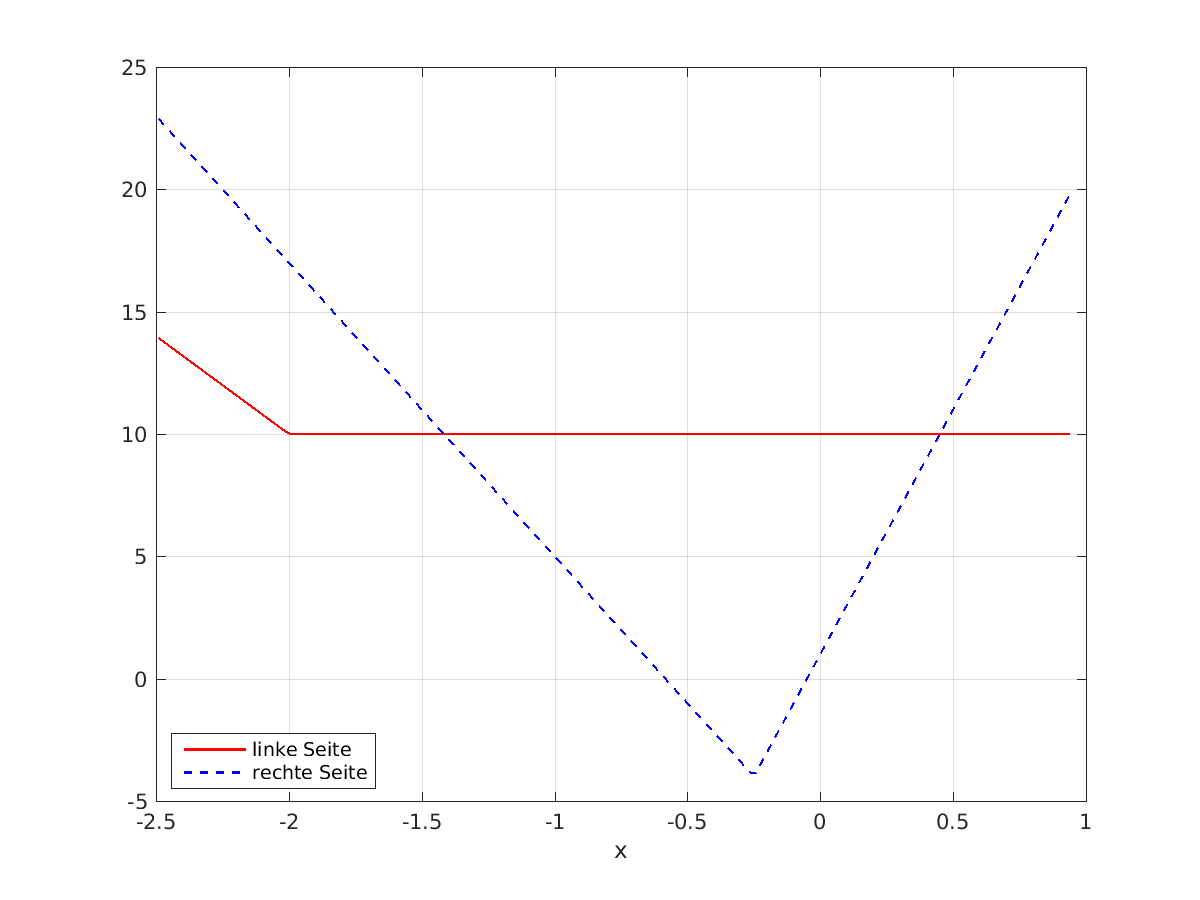
\includegraphics[width=0.8\linewidth]{Abb_zur_Ag_autogenerated_ineq_11.png} \end{center}
 
\else\relax\fi
 \end{MAufgabe}